\documentclass[fleqn,14pt]{article}

\usepackage[letterpaper,margin=0.75in]{geometry}

\usepackage{amsmath}
\usepackage{booktabs}
\usepackage{graphicx}
\usepackage{listings}
\usepackage{fancyhdr}
\usepackage{standalone}
\usepackage{pgfplots}
\usepackage{float}
\usepackage{csvsimple}
\usepackage{hyperref}
\usepackage{biblatex} %Imports biblatex package

% Bibliography
\addbibresource{all.bib}

% \include{data/reaction-time.csv}
 
\pgfplotsset{compat = newest}

\setlength{\parindent}{1.4em}

\pagestyle{fancy}


\begin{document}

\lstset{
  language=Python,
  basicstyle=\small,          % print whole listing small
  keywordstyle=\bfseries,
  identifierstyle=,           % nothing happens
  commentstyle=,              % white comments
  stringstyle=\ttfamily,      % typewriter type for strings
  showstringspaces=false,     % no special string spaces
  numbers=left,
  numberstyle=\tiny,
  numbersep=5pt,
  frame=tb,
}

\title{Lab Report}
\date{}
\def\theinstructor{Benjamin Koltai}



\author{Sidney Pauly}
\def\theuoastudentid{52104132}

\makeatletter

\let\thetitle\@title
\let\theauthor\@author
\let\thedate\@date


\makeatother




\fancyhf{}
\fancyhead[L]{Name: \theauthor}
\fancyhead[C]{ID: \theuoastudentid}
\fancyhead[R]{Instructor: \theinstructor}


% \maketitle

\begin{titlepage}
  \begin{center}
    \Large
    \textbf{\thetitle}
        
    \vspace{0.4cm}
    \large
    PX1015 - Experiment 5 - Counting and Timing
        
    \vspace{0.4cm}
    \textbf{\theauthor}\\
    \textbf{\theuoastudentid}

       
    \vspace{0.9cm}
    \textbf{Abstract}
  \end{center}
  The following experiments explore how digital counting can be used to collect very
  precise data from experiments.
  The experiments especially focus on how to use the digital counters to measure time intervals
  very precisely. This enabled measuring human reaction time,
  the frequency up to which a human can discriminate between flashes of a LED and the acceleration 
  of a falling ball. With this goal in mind, the experiment also lead
  to an exploration of the fundamentals that go into digital counting, like wiring
  up a circuit, using a function generator, using an oscilloscope and
  understanding how digital counters work.

  \vfill

  \begin{center}

    University of Aberdeen\\
    Scotland\\
    UK\\
    \thedate
    \vspace{0.4cm}
    \url{https://github.com/sidney-pauly/papers}
  \end{center}
\end{titlepage}




% \begin{lstlisting}
% class Node:
%     def __init__(self,scheduler):
%         self.scheduler = scheduler

%     def handle_message(self,t,message):
%         print "Received at",t,':',message.body
%         if message.times < 3:
%             self.scheduler.add(t+1.5, message, self.handle_message)
%         message.times += 1
% \end{lstlisting}

\section{Introduction}
Our modern world is heavily relying on electrical circuitry. More specifically integrated ones (ICs).
A common way how such circuits operate is by utilizing a clock cycle. I. e. they do something every pulse.
Today the most advanced circuits (computers) run with frequencies (clock cycles per second) of up to
a few billion Hz (Ghz). A very basic circuit that can make use of a such cycles is a counter.
It simply counts +1 for every
pulse it receives. If the pulses are at a constant frequency this method can also be used to measure time.

\section{Theory}
\subsection{Electrical}

When wiring up any electrical circuitry some base theory is needed. First there is Ohms law,
it tells us how resistance,
Current and Voltage are related as such:
$$
I = \frac{V}{R}
$$
The law is helpful, whenever we need to figure out how to wire up a component that has limits
on either the current or voltage it can handle,
or how a resistor (i.e. any consumer) will affect the circuit. It tells us that the current
is inversely proportional to the resistance. Thus if we want to decrease the current we need
to increase the resistance.\\
Then there is also the Laws on how to combine resistors:
\newline
\newline
Series:
$$
R_T = R_1 + R_2
$$
Parallel:
$$
\frac{1}{R_T} = \frac{1}{R_1} + \frac{1}{R_2}
$$
They tell us that if we combine resistors in parallel the overall resistance will decrease.
On the other hand if they are combined in series their resistance will add up.

\subsection{Binary counting}
Digital circuits have two basic states: off and on (0 and 1). They can’t handle other values.
In order to count base 10 (0-9) is therefore unusable and and the usage based on base 2/binary (0-1) is
necessary.
One digit of a binary number is called a bit.\\
Some examples for binary numbers with
their decimal counterparts:

\vspace{0.5cm}
\begin{tabular}{lc}
  Binary & Decimal\\
  \midrule
  $0000\_0100$ & 4\\
  $0000\_1000$ & 8\\
  $0001\_1000$ & 24\\
\end{tabular}
\vspace{0.5cm}


Translating from binary to decimal is easy. It can be done with the following formula:
$$
d=n_0\ast2^0+n_1\ast2^1+\ldots+n_m\ast2^m
$$
Where n, the corresponding binary digit.

\subsection{Kinematics}

Furthermore some Kinematic equations will be used to calculate the acceleration
(constant) of a falling object. Using two section, within which the objects velocity is measured,
the acceleration can be calculated as such:\\
\\
Average velocity
$$
v_{avg}=\frac{l}{t}
$$

We can then take the difference between $v_1$ and $v_2$ to get $\Delta v$ as well as the difference between
$t_1$ and $t_2$ to get $\Delta t$.\\
\\
Therefore
$$
a = \frac{\Delta v}{\Delta t}
$$
Plugging everything in:
$$
a = \frac{2(\frac{l_2}{t_2}-\frac{l_1}{t_1})}{t_1+t_2}
$$

\section{Experimental Procedure}
\subsection{Wiring up an LED}
To test and verify the electrical setup the first step was to wire up a LED. For quick reconfiguration of
the circuits a breadboard was used. To operate a LED and do so safely two things have to be taken into account
\begin{enumerate}
\item Direction: LEDs are diodes (LightEmittingDiode) so they only let electricity pass in one direction
\item Current: LEDs can only be used up to a certain current, beyond that they gets damaged.
\end{enumerate}
Finding out the direction was done by testing which way it lit up. This can be done as the LED is not
damaged
if wired up the wrong way around. To limit the current flowing through the LED a resistor wired up in
parallel was used. As can be seen from $I = \frac{V}{R}$ the current can be decreased by increasing the
resistance. The documentation on the LED called for a $330\Omega$ resistor. As such a resistor was not
available, instead two $160\Omega$ where used in series instead. After connecting a 5 volt power supply
the LED lit up successfully.

\subsection {Function generator and Oscilloscope}
The next step was trying out the function generator. As it had a 5 volt output as well it could be used as
a direct substitute for the power supply. As the circuits used later needed square waves to work properly,
that setting was also chosen to test the LED. To verify that everything worked properly a low, human
perceivable frequency of 1Hz was chosen. After turning on the function generator the LED started
to blink.
\newline
\newline
Next the oscilloscope was brought out to take a closer look at the output of the function generator. It
was wired up as illustrated in the manual:
\begin{figure}[h]
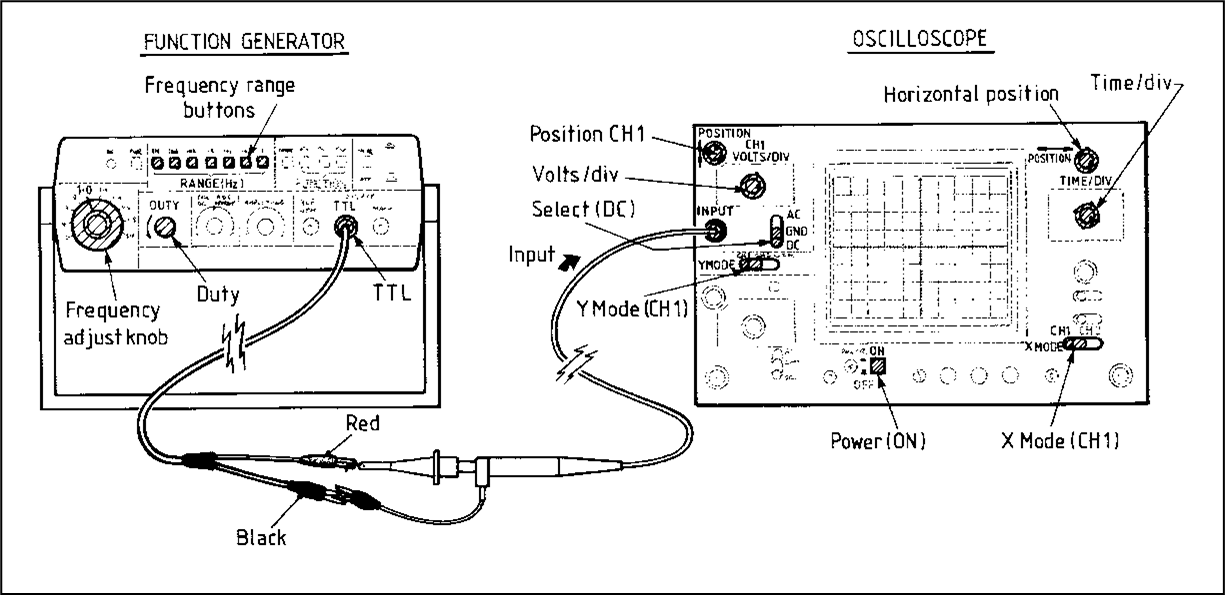
\includegraphics[width=16cm]{images/Oscilloscope.png}
\caption{Function Generator wired up to Oscilloscope \cite{ross}}
\label{fig:figure1}
\end{figure}

First the Time/div knob was set to a very high value, this resulted in just a spot showing on the
oscilloscope. By centering (Position CH1) that point (0V) the oscilloscope could be calibrated. After that the
Volts/div slider was set such that it lay within the 5V range of the function generator. This resulted
in two spots showing. In a third step the Time/div slider was set such that the time interval was close
to what the function generator was producing as an output. The result was a square wave showing on the
oscilloscope:

\begin{figure}[H]
  \centering
  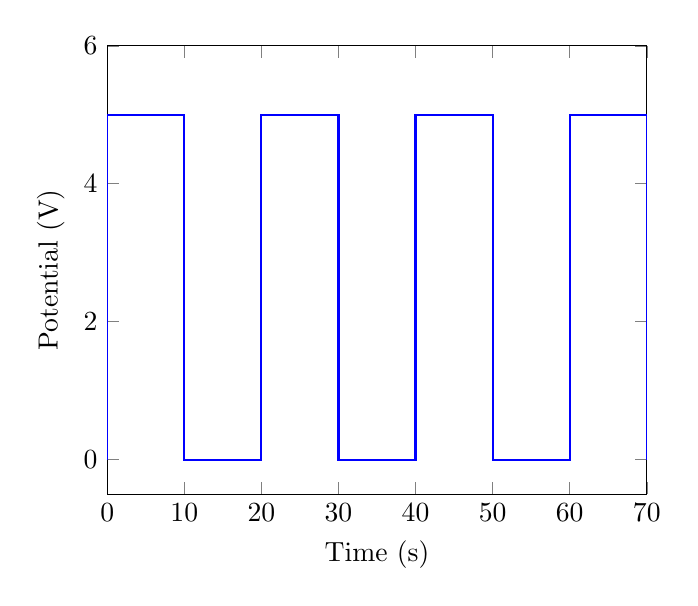
\begin{tikzpicture}
 
    \begin{axis}[
        ylabel={Potential (V)},
        xlabel={Time (s)},
        xmin = 0, xmax = 70,
        ymin = -0.5, ymax = 6]
        \addplot+[thick,mark=none,const plot]
        coordinates
        {(0,0) (0,5) (10,0) (20,5) (30,0) (40,5) (50,0) (60,5) (70,0)};
    \end{axis}
     
  \end{tikzpicture}
  \caption{Idealized plotted square wave}
  \label{fig:figure2}
\end{figure}

Increasing the frequency of the function also changed how long each of the pulses on the oscilloscope where showing.
This setup now let us take a reading on what frequency the human eye can perceive. To do so the
frequency was set to 100Hz (No perceivable flickering), and slowly lowered until flickering could be perceived.

\subsection{Counting}
To count different counting circuits where wired up instead of the LED. They needed a constant Voltage
of 5V so the power supply was used again. All of the different counter circuits offered two pins to connect
a clock. The function generator was connected to those pins as such a timing device. The first circuit had
just two buttons start and reset without any additional pins as well as a bar of LEDs to show the current
count. With it the overall setup was confirmed to be working. 
\newline
\newline
Afterwards the a counting device with a
7-segment display was connected. It offered an additional switch to either use the direct output
of the counting IC or put it through a binary to BCD translation IC. BCD stands for  Binary-Coded-Decimal.
BCD uses 4 bits per decimal digit to represent it. 4 bits are used as $2^4=16 > 9$. 
\newline
\newline
Proceeding we wired up a circuit that counted the number of pulses within a given time period (switchable between
0.1s, 1s or 10s). By connecting the function generator again we could test how many pulses where generated by
it in a given second.
\newline
\newline
Last a counting device with four 7-segment displays was connected, it could count up to 9999 ($10^4$). In
addition it also had a start, stop and a reset button with electrical pins, that if grounded also activated
the corresponding action. The stop button was then wired to a hand-held thumb-actuated button. The function
generator was then set to a 1000Hz such that a value of 1 on the counter would represent 1ms. One person then
covered up the start switch with their hand, reset the counter and prepared to press it. The other person
held the stop button, their job was it to press it as soon as they could see the counter starting to count.
This way the reaction time of the person holding the stop-button could be tested. We both recorded our
reaction-times four times varying the time the person had to wait before the start button was pressed.

\subsection{Measuring Gravity}
With the counting circuits setup and verified we could proceed to use them to measure the gravitational
acceleration on different objects. To do so a drop tower with three gates was used. Additionally two of the
previously introduced four 7-segment counters where used. The gates of the tower where then wired up such
that gate one was connected to the start pin of the counter one, gate 2 to the stop pin of counter one as
well as the start counter of counter two and gate three to the stop pin of counter two. Thus creating a
setup that could count the number of pules passing while a object traveled between the respective gates.
By setting the function generator to produce an output of 1000Hz this could then be translated into time.
With this setup different objects where dropped down the tower. Balls of two sizes and 4 different materials
where used as well as a small pen as an object with minimal air resistance. To get additional precision
the actual produced frequency displayed on the function generator was also recorded to apply it as a
later correction. To improve accuracy further a run with done with the function generator set to 10,000Hz.

\section{Experimental Results}

\subsection{Human perceivable frequencies}

\vspace{0.5cm}
\begin{tabular}{lc}
  Person & Frequency (Hz)\\
  \midrule
  Sidney & 36\\
  Bray & 30\\
\end{tabular}
\vspace{0.5cm}

\subsection{Digital Counting}
\paragraph{BIN/BCD circuit}
While testing the BIN/BCD switchable counting circuit it was observed that the 7-segment display did not
go through the numbers correctly all of the time. If the switch was set to BCD the counting worked correctly
with the display going form 0 to 9 and then resetting. Setting the switch to BIN this did not work properly.
The display was instead counting up to 6 and then did show different numbers in a random seaming way.
\paragraph{Function Generator output verification}
When connecting the function generator to the 1s resetting counter, we set different frequencies on
the function generator and observed what the counter counter showed. The observation where as follows:

\begin{enumerate}
  \item When changing the frequency on the oscilloscope it took a while for the number of counts to
  stabilize.
  \item When pressing any of the buttons or moving the cables of the counting circuit the same happened
  \item Once settled the counter showed the same value as the reading on the oscilloscope up to 1 count
  of difference
\end{enumerate}

\subsection{Reaction Time}

\vspace{0.5cm}
\begin{tabular}{l|ccccc|cc}
  Person & 1 & 2 & 3 & 4 & 5 & Average & Standard Deviation\\
  \midrule
  Sidney & 242.3 & 225.5 & 156.5 & 163 & 228.7 & 203.2 & 40.2\\
  Bray & 189.5 & 330.5 & 252.9 & 150.2 & 171.1 & 218.84 & 73.3\\
\end{tabular}
\vspace{0.5cm}

\subsection{Gravity}

\begin{tabular}{lcccccc}
  Material & $t_0$ & $t_1$ & Correction & $t_{0_{corrected}}$ & $t_{1_{corrected}}$ & g\\
  \midrule
  Rubber & 0.175 & 0.1 & 0.996015936 & 0.174302789 & 0.099601594 & 9.425604156\\
  Wood & 0.179 & 0.1 & 0.996015936 & 0.178286853 & 0.099601594 & 9.567281072\\
  Plastic & 0.182 & 0.104 & 0.996015936 & 0.1812749 & 0.103585657 & 8.714500884\\
  Wood small & 0.18 & 0.1 & 0.996015936 & 0.179282869 & 0.099601594 & 9.600152381\\
  Glass small & 0.181 & 0.099 & 0.996015936 & 0.180278884 & 0.098605578 & 9.884637057\\
  Metal & 0.181 & 0.099 & 0.996015936 & 0.180278884 & 0.098605578 & 9.884637057\\
  Glass  & 0.18 & 0.099 & 0.996015936 & 0.179282869 & 0.098605578 & 9.853528837\\
  Dart & 0.1441 & 0.097 & 1.005025126 & 0.144824121 & 0.097487437 & 8.302050935\\
  Metal (10kHz)& 0.1765 & 0.0981 & 1.005025126 & 0.177386935 & 0.098592965 & 9.794882365\\

\end{tabular}
\vspace{0.5cm}


\section{Discussion and Analysis}

\subsection{Human perceivable frequencies}
Here we don't have a lot of data so a real analysis is not possible. Still some interesting things can be said.
The first observation made was that there is no hard boarder between no flickering and flickering. There is analysis
area inbetween where there is no flickering perceived, but the LED is also not percived as being continuously on.
The perceived effect, might, in appearance, be comparable to candle light. There is flickering, but not with
a frequency of the set 20Hz-40Hz more in the range of 5-10Hz. There might be to possible explanations:

\begin{enumerate}
  \item There is an error in the electronics and the LED sometimes stays of for longer thant what is configured
  \item Past a certain frequency the flashes are to fast for a person to perceive them. Instead they only
  catch e.g every other flash. This could be similar to a shutter in a camera that depending on the set frequency
  either catches the Light being on or off. Of course human eyes have no shutter, but this could be something
  happening in the brain.
\end{enumerate}

Hypotheses one seems to be a bit more unlikely. This is because these supposed slip-ups are not observable
at other frequencies. Also the other examinations with the oscilloscope did not reveal anything of the like.

\subsection{Digital Counting}
While testing the 7-segment display counter wired behavior was observed while the switch was set to BIN.
A possible explanation is that the 7-segment display driver IC expects a BCD input and thus if that translation
does not happen, still assumes the input is BCD. This can be confirmed by looking at what the 7-segment display
would output in such a case:

\vspace{0.5cm}
\begin{tabular}{lccc}
  Binary & BCD & Actual Decimal & Displayed Decimal\\
  \midrule
  $0000\_0001$ & 0001 & 1 & 1\\
  $0000\_0010$ & 0010 & 2 & 2\\
  $0000\_0011$ & 0011 & 3 & 3\\
  $0000\_0100$ & 0100 & 4 & 4\\
  $0000\_0101$ & 0101 & 5 & 5\\
  $0000\_0110$ & 0110 & 6 & 6\\
  $0000\_0111$ & 0111 & 7 & 7\\
  $0000\_1000$ & 1000 & 8 & 8\\
  $0000\_1001$ & 1001 & 9 & 9\\
  $0000\_1010$ & 0001 0000 & 10 & 2\\
  $0000\_1011$ & 0010 0000 & 11 & 3\\
  $0000\_1100$ & 0011 0000 & 12 & 4\\
\end{tabular}
\vspace{0.5cm}

It can be seen that as soon as the counter reaches double digits it would be different from the actual
number. While it can't be confirmed that this is the exact behavior exhibited by the counter (as the
sequence produced by it was not recorded), it is likely that this or something similar happened.\\

\subsection{Reaction Time}
Again with the limit of only having two human test subjects the results of the experiment are quite limited.
Also it has to be noted that the recorded numbers might differ slightly, because of the jitter of the function
generator that could be observed if any of the buttons where being pressed. This can likely be neglected
here as the jitter seamed to be happening equally in both directions and should therefore average out
over the runs. Additionally the standard deviation is in any case a lot higher than what the jitter alone
could explain. This is because the jitter was observed to be in the single millisecond domain, while the
standard deviation is in the 100 millisecond domain.\\
\\
Keeping this in mind there are again some interesting observations to be made. First the reaction time of 20
year old test subjects seams to lie in the 200-220 millisecond range. This is close to the value stated in
online resources \cite{wiki} . Also noteworthy is the high standard deviation. It shows that human reaction time is not
consistent. This might have different reasons, one of them could be if the subject focuses on the LED
or is distracted. Another factor could be the waiting time until the LED lights up. It could happen that the
subject involuntarily loses interest after a while. It would definitely be insightful to repeat the experiment
with more test subjects, with more trials spread over the a longer time span.

\subsection{Gravity}
The last experiment seams to be the one that should produce the most precise results as no humans as test
subjects are involved.
Besides that there are likely some caveats that might still contribute to not getting precise measurements.\\
One factor could again be the effects of the aforementioned jitter in the function generator.
This is a problem because
$$
\Delta a \propto \frac{1}{\Delta t^2}
$$
As a result any slight variatons in the measured time have a big impact on the measured acceleration. To mimize
this problem we added a correction term to our calculations. It states how the exact frequency that the
function generator displayed during the specific trial. This correction can only account for a general offset,
not for the jitter induced by the falling object triggering the gates.\\
Other factors hindering the precision of the experiment are the imprecise measurement of the tube length (only
accurate to $10^-1m$) as well as the tube itself potentially trapping air and thus causing a air cushion to
be formed. \\
\\
Also potentially affecting the results is the time resolution of the counter. With the function generator
set to 1kHz only time-steps of 1ms can be recorded. To get more precision, we set the function generator
to 10kHz for the last trial, giving us a 10x improved time resolution. It again is debatable if that improved
things, as the aforementioned jitter might at this point be a lot bigger than the smallest measurable.
\\
If this experiment is repeated, the most important thing is to reduce the jitter, this might be possible to
do by modifying the circuits (e.g. adding a capacitor), so that any electrical effects induced by the switching
get reduced. Additionally doing multiple trials with the same object might improve the situation as well.\\
\\
The results itself are on a first look not surprising. Heavier materials, as well as bigger objects fall faster.
This is easily explained by a looking at the formulas governing the fall:\\
\\
Air resistance:
$$
F_a \propto A
$$
Force due to gravity:
$$
F_g = g m
$$
as the mass of a sphere is given by
$$
m = \rho \frac{4}{3} \pi r^3
$$
thus,
$$
F_g = g \rho \frac{4}{3} \pi r^3
$$
while the area is described by
$$
A =  4 \pi r^2
$$
thus,
$$
F_a \propto r^2
$$
while
$$
F_g \propto r^3
$$
therefore $F_a >> F_g$ for big $r$
and
$$
F_g \propto \rho
$$
(With $F_a$ as air resistance, $F_g$ as force due to gravity and
$F_{total} = F_g - F_a$)\\
\\
While this part of the result is confirmed by theory, another detail is a lot harder to explain. In some
of the trials the measured acceleration was higher than what is commonly quoted as $g$ in Aberdeen ($9.1ms^-2$).
This might point to a systematical error of the experiment that shifts all of the measured results up, above
the actual present acceleration. Curiously, the last trial where the function generator was set to 10kHz was
a lot closer to the expected value of $g$ (note that a big metal ball was used, thus reducing the effect of 
air resistance as shown). Without making more measurement it is not conclusive if this was just a statistical
fluke or actually the result of the improved time resolution.

\section{Conclusion}
Overall it could be observed that using electronic circuits and counting devices, allows for a wider range
of experiments to be conducted. This is especially true for processes that happen fast and can thus not
be fully grasped by mere unaided observation. It is also clear that electronic counting/measuring allows
for a lot higher time-resolution while conducting experiments. This is highlighted by the fact that the
highest achievable time-resolution within the experiment was 0.1ms (10kHz), while the highest time-resolution
that was achieved by a human lay only at around 33ms (30Hz). As noted it might even be possible to improve
this with better electronics and by conducting more runs.

\printbibliography

\end{document}